% !TEX TS-program = LuaLaTeX+shellescape
% !TEX encoding = UTF-8 Unicode
\RequirePackage{luatex85}
\documentclass[crop=true]{standalone}
\usepackage{pgfplots}
\usepgfplotslibrary{fillbetween}
%\usetikzlibrary{angles}
\pgfplotsset{compat=1.15}
%\pdfminorversion=5 % to allow compression
%\pdfobjcompresslevel=5
%\pdfcompresslevel=14
%\pgfplotsset{
%	layers/my layer set/.define layer set={background,main,foreground}{},set layers=my layer set,}

\begin{document}
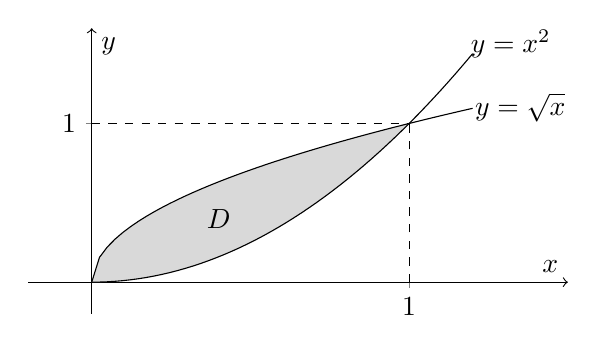
\begin{tikzpicture}[baseline]
\begin{axis}[
axis lines = middle,
unit vector ratio*=2 1 1,
scale=1.0, xmin=-0.2, xmax=1.5, ymin=-0.2, ymax=1.6,
%grid = major,
xtick={0,1},
ytick={0,1},
xticklabels = {0,1},
yticklabels = {0,1},
xlabel=$x$,
ylabel=$y$,
axis line style = {->},
]
\addplot[name path=up,samples=50,domain=0:1.2]{x^2};
\addplot[name path=below,samples=50,domain=0:1.2]{sqrt(x)};
%\addplot[name path=xaxis,domain=0:2]{0};
%\draw[thick](axis cs:1,0) -- (axis cs:1,3);
\addplot[gray!30]fill between[of=up and below,soft clip={domain=0:1}];
%\draw[thick](axis cs:0.2,0.4) rectangle (axis cs:2.4,2.3);
%\coordinate (A) at (axis cs:1,0);
%\coordinate (B) at (axis cs:0,0);
%\coordinate (C) at (axis cs:0.86602540378,0.5);
%\draw[] (axis cs:0.3,0.2) -- (axis cs:0.3,2) -- (1.7,2) -- (axis cs:1.7,0.2) -- cycle;
\draw[thin,dashed] (axis cs:1,0) -- (axis cs:1,1);
\draw[thin,dashed] (axis cs:0,1) -- (axis cs:1,1);
%\draw[thin,dashed] (axis cs:0,0.2) -- (axis cs:0.3,0.2);
%\draw[thin,dashed] (axis cs:0,2) -- (axis cs:0.3,2);
%\pic[draw,angle radius=0.5cm,angle eccentricity=1.5]{angle = A--B--C};
\node at (axis cs:0.4,0.4){$D$};
\node at (axis cs:1.32,1.5){$y=x^2$};
\node at (axis cs:1.35,1.1){$y=\sqrt{x}$};
\end{axis}
\end{tikzpicture}



\end{document}